\section{Architecture Overview}
\label{socksdirect:sec:architecture}


\begin{figure}[t!]
	\centering
	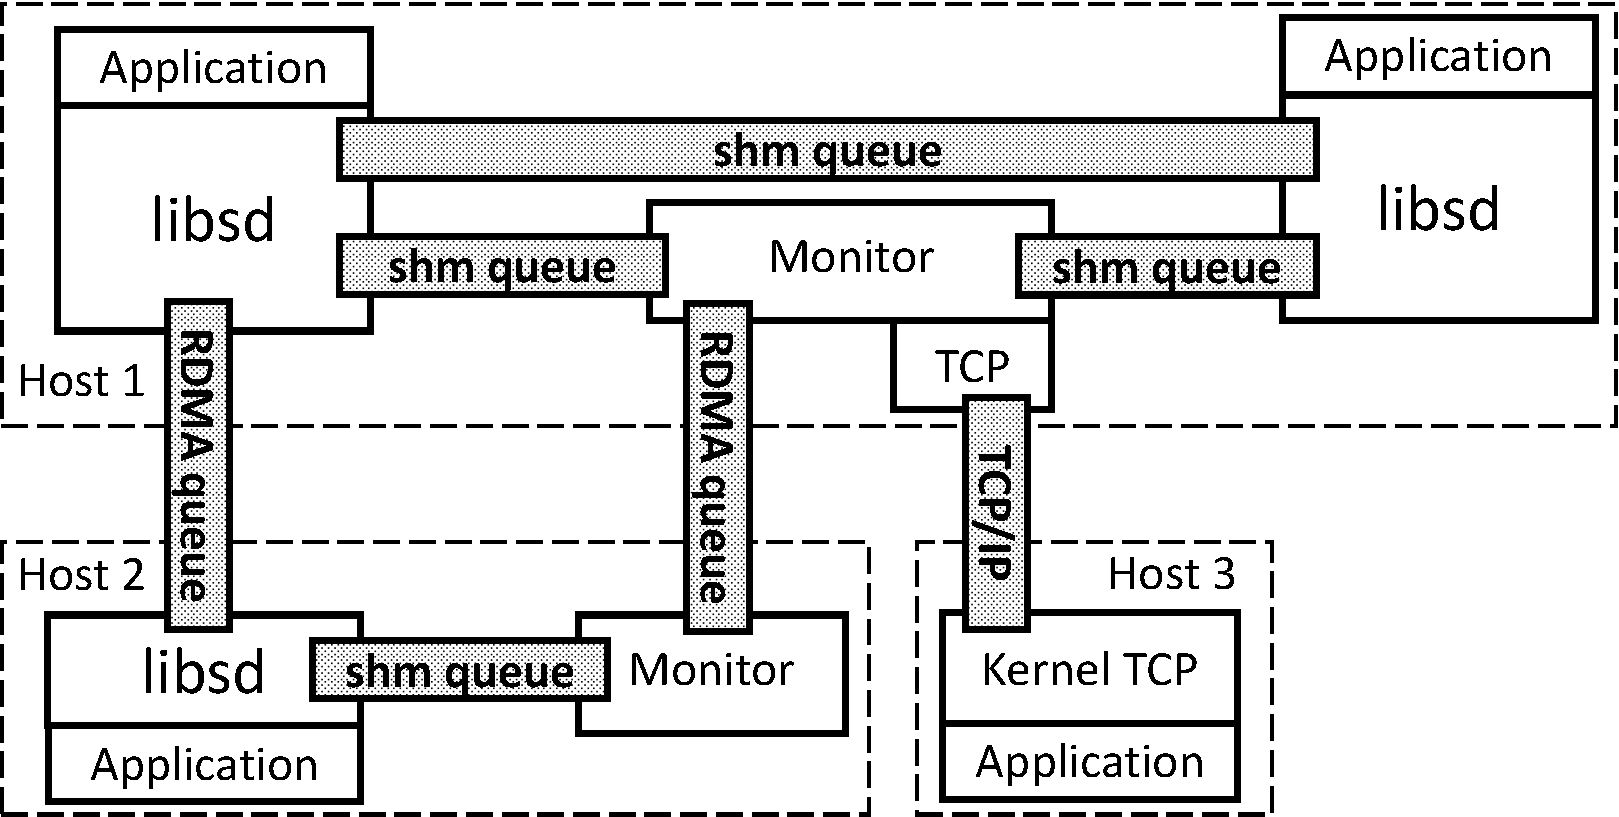
\includegraphics[width=0.8\textwidth]{images/architecture_new}
	
	\caption{Architecture of \sys{}. Host 1 and 2 are RDMA capable, while host 3 is RDMA incapable.}
	\label{socksdirect:fig:architecture}
	\vspace{5pt}
\end{figure}


\iffalse
\begin{figure}[t!]
	\centering
	\subfloat[Traditional queue structure.]{
		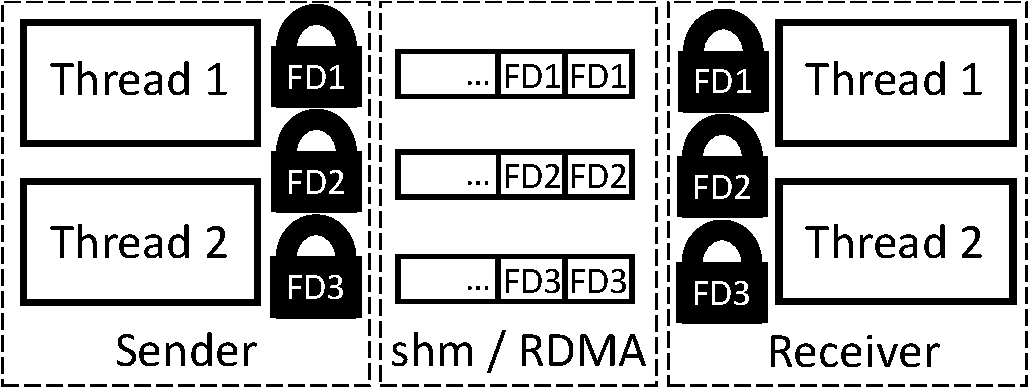
\includegraphics[width=0.4\textwidth]{images/fork_linux}
	}
	
	\subfloat[\sys{} queue structure.]{
		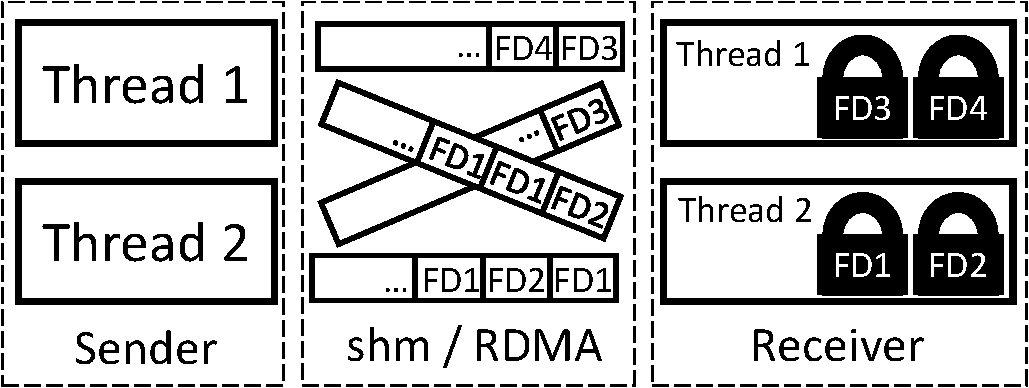
\includegraphics[width=0.4\textwidth]{images/fork_rdwr}
	}
	
	\caption{Comparison of queue structures. Assume sender and receiver each has two threads. First, \sys{} creates peer-to-peer queues between each pair of sender and receiver threads. Rather than protecting the queue with locks, we designate each FD to a receiver thread to ensure ordering. Second, data from all connections (FDs) are multiplexed through a shared queue, instead of one queue per FD.}
	\label{socksdirect:fig:fork-rdwr}
\end{figure}
\fi


%As shown in Figure~\ref{socksdirect:fig:architecture}, the core component of \sys{} is a user-space library \libipc{}.

To simplify deployment and development~\cite{andromeda}, as well remove kernel crossing overhead, we implement \sys in user space rather than kernel.
To use \sys, an application loads a user-space library \libipc{} by setting the \texttt{LD\_PRELOAD} environment variable. \libipc{} intercepts all Linux APIs in standard C library that are related to file descriptor (FD) operations. It uses a \emph{FD remapping table} to distinguish socket FDs from kernel FDs (e.g. file and devices), implements socket functions in user space and forwards others to the kernel.
From a security point of view, because \libipc{} resides in the application address space, we cannot trust its behavior. For example, a malicious application may bypass firewall policies if it is enforced in \libipc{}. Furthermore, TCP port is a global resource that needs allocation~\cite{lin2016scalable,nsdi19freeflow}. Therefore, we need a trusted component outside \libipc{} to enforce access control and manage global resources.

To this end, we design a \emph{monitor} daemon at each host to coordinate control plane operations, e.g., connection creation. The monitor is a system service. In each host, all the applications loading \libipc{} must establish a shared memory (SHM) queue with the host's monitor daemon, forming the control plane. On the data plane, applications build peer-to-peer queues to communicate directly, thus relieving the burden of the monitor daemon. Figure~\ref{socksdirect:fig:architecture} shows the architecture of \sys{}.



%To this end, we regard processes as a shared-nothing distributed system that communicates through message passing.
%We design a secure control-plane protocol between applications and the monitor, and a data-plane protocol between applications.

To achieve low latency and high throughput, \sys{} uses SHM for intra-host and RDMA for inter-host communication.
Each socket connection is mapped to a SHM queue or RDMA QP.
A SHM or RDMA QP is marked by a unique token, so other non-priviledged processes cannot access it.
A socket send operation is translated to a SHM or RDMA write operation to the socket buffer on the remote endpoint.

For \emph{intra-host} communication, the communication initiator first sends a request to the local monitor, then the monitor establishes a shared memory queue between the two applications (possibly in different containers). Afterwards the two applications can communicate directly.


%During initialization, \libipc{} connects to the local monitor via a shared memory queue.
%To enforce access control policies and support overlay networks, % and load balance new connections to multiple listeners, 
%connection request is always sent to the local monitor.
%For local peers, the monitor just construct a shared memory queue between the two applications , %so they can communicate directly.

For \emph{inter-host} communication, the monitors of two hosts are both involved. When an application connects to a remote host, its local monitor establishes a regular TCP connection and detects whether the remote host supports \sys{}.
%When the monitor connects to another host for the first time\RED{Why we need to connect two monitors?}, it establishes a regular TCP connection and detects whether the remote host supports \sys{}.
If so, it establishes an RDMA queue between the two monitors, so that future connections between the two hosts can be created faster. The monitor at the remote side dispatches the connection to the target and helps the two applications establish an RDMA queue, as between host 1 and 2 in Figure~\ref{socksdirect:fig:architecture}. If the remote host does not support \sys{}, it keeps using the TCP connection, as between host 1 and 3 in Figure~\ref{socksdirect:fig:architecture}. The detailed connection management protocol is presented in Sec.~\ref{socksdirect:subsec:connection-management}.

To ensure thread safety and avoid locking, as well support fork and container live migration, we optimize for the common case where only one pair of send and receive threads are active, while ensure correctness in all cases (Sec.~\ref{socksdirect:subsec:fork}).
%With the control plane mechanisms above, a socket connection is mapped to a queue with a pair of active sender and receivers.
%The data plane aims to implement the queue efficiently.
To remove buffer management overheads, we design a ring buffer that only requires (amortized) one RDMA write operation per inter-host message and one cache migration per intra-host message (Sec.~\ref{socksdirect:subsec:lockless-queue}).
We further design a zero copy mechanism that removes data copy on both send and receive side for large messages (Sec.~\ref{socksdirect:subsec:zerocopy}).
Finally, Sec.~\ref{socksdirect:subsec:process-mux} presents our event notification mechanism.

%In order to remove synchronization overhead for multi-threaded applications, we treat each thread as a separate process.
%%Although threads in a process share memory, we use thread-specific storage for most states in \libipc{}.
%For two communicating applications, we create peer-to-peer queues between each pair of sender and receiver threads to avoid synchronization cost of contending on the same queue.
%In Sec.~\ref{socksdirect:subsec:fork}, we present the peer-to-peer queue design that preserves FIFO ordering semantics and avoids starvation, especially when a process forks or creates a new thread.
%To maintain performance with many concurrent connections, rather than creating separate queues for each connection, we multiplex data from all connections through one queue.
%In Sec.~\ref{socksdirect:subsec:multiplex-conn}, we present the design of multiplexed queue that avoids head-of-line blocking and supports fetching data from any multiplexed connections.

%Inspired by Unikernels~\cite{madhavapeddy2013unikernels}, we move networking and IPC functions from the kernel to user space. Similar to existing works~\cite{peter2016arrakis,jeong2014mtcp,libvma}, we leverage multiple queues in modern NICs to enable user-space direct access to network. %The kernel is still responsible for process creation, scheduling, virtual memory and device management, but no longer on the critical path of performance.
%To maintain compatibility with existing Linux applications, we design a user-mode library \libipc as a drop-in replacement of the system call wrappers in the GNU C library (glibc). \libipc{} implements network socket functions in user mode, and adds a wrapper to other system calls to track process creation and memory allocation. \libipc{} is not considered a secure domain, as it shares memory space with the application. When \libipc{} is loaded, it creates a Linux native \textit{bootstrap socket} to the \textit{monitor} daemon, then creates a shared memory queue to the monitor.

%Even though multiple threads in the same process share memory space, we still treat each thread as a separated process and use thread-specific storage to store states in \libipc. In the following text, unless explicitly mentioned, we use a ``process'' to refer to a regular process or a thread.

\section{Design}
\label{socksdirect:sec:design}


\subsection{Lock-free Socket Sharing}
\label{socksdirect:subsec:fork}


\begin{figure}[t!]
	\centering
	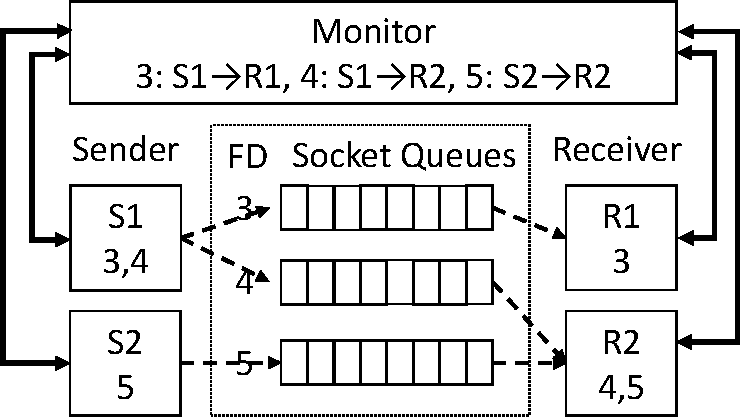
\includegraphics[width=0.6\textwidth]{images/queue_arch}
	
	\caption{Lock-free socket sharing with two sender and two receiver threads. Dashed arrows indicate the active sender and receiver of each socket. Each thread tracks its active sockets and communicates with the monitor via an exclusive queue.}
	\label{socksdirect:fig:queue-arch}
\end{figure}

Most socket systems acquire a per-FD lock to enable threads and processes share a socket (Sec.~\ref{socksdirect:subsec:per-operation-overhead}).
Previous work~\cite{boyd2010analysis,clements2015scalable} suggests that many socket operations are not commutable and synchronizations cannot always be avoided.
We leverage the fact that SHM message passing is much cheaper than locking~\cite{roghanchi2017ffwd}, and use message passing as the exclusive synchronization mechanism.

Logically, a socket is composed of two FIFO \emph{queues} in opposite directions, each with multiple concurrent senders and receivers.
Our aim is to maximize the common-case performance while preserving the FIFO semantics.
We make two observations: First, fork and thread creation are infrequent in high performance applications because of their high cost.
Second, it is uncommon that several processes send or receive concurrently from a shared socket, because the byte-stream semantics of socket makes it hard to avoid receiving partial messages.
%If the application needs to send or receive concurrently, message brokers~\cite{hintjens2013zeromq,rabbitmq2017rabbitmq,kreps2011kafka} are typically used.
The common case is that the application implicitly migrates a socket from one process to another, e.g. offload a transaction from master to a worker process.

\iffalse
Based on the observations, we propose the following requirements:

\begin{enumerate}[noitemsep,nolistsep]
 \item \textbf{Synchronization-free.} With multiple senders and receivers, if only one pair of sender and receiver is active, no synchronization should occur.
 \item \textbf{Multi-sender scalability.} Multiple processes may send data concurrently through a shared socket. With multiple active senders and a single receiver, if the receiver is not a bottleneck, the throughput should scale.
 \item \textbf{Self-stabilization.} Certain operations (\textit{e.g.} \texttt{fork}) may slow down the system temporarily, but after that the performance should converge back to normal.
\end{enumerate}

For compatibility with Linux semantics, we also need to ensure message ordering and liveness:
\begin{enumerate}[noitemsep,nolistsep]
\item \textbf{Single receiver ordering.} For a specific pair of sender and receiver, the received messages have the same ordering as they were sent.
\item \textbf{Multiple receiver ordering.} The order of \texttt{send} and \texttt{recv} operations for one sender and multiple receivers should be linearizable. If receiver $R_1$ receives $D_1$ before receiver $R_2$ calls \texttt{recv} and gets $D_2$, we guarantee that $D_1$ is sent before $D_2$.
\item \textbf{Deadlock-free.} If a socket buffer is not empty when \texttt{recv} is called by one or more receivers, at least one receiver should get data.
\item \textbf{Starvation-free.} If a sender keeps sending, any receiver trying to \texttt{recv} will eventually get some data.
\end{enumerate}
\fi

Our solution is to have a \emph{send token} and a \emph{receive token} per \emph{socket queue} (one direction of a socket).
Each token is held by an \emph{active thread}, which has the permission to send or receive.
So there is only one active sender thread and one active receiver thread at any point of time.
The socket queue is shared among the threads and processes, which allows lock-free access from one sender and one receiver (details will be discussed in Sec.~\ref{socksdirect:subsec:lockless-queue}).
When another thread wants to send or receive, it should request to \emph{take over} the token.

%\RED{Need performance comparison in a figure.}

The details for each type of operations are as follows: %four types of operations: a) data transmission (\texttt{send} and \texttt{recv}), b) adding new senders and receivers (\texttt{fork} and thread creation), c) container live migration, and d) connection close.

\subsubsection{Send/Recv Operation}
\label{socksdirect:subsubsec:fork_rdwr}
\quad

When a thread does not have the send token but wants to send through the socket, the inactive thread needs to \emph{take over} the token.
If we create a direct communication channel between the inactive and active threads, there will either be peer-to-peer queues with number quadratic to the number of threads, or a shared queue with locking.
To avoid both overheads, we use the monitor daemon as a proxy during the \emph{take over} process.
This message passing design also has the benefit that sender processes can be on different hosts, which will be useful in container live migration.

The take over process is as follows:
The inactive sender sends a \emph{take over} command to the monitor, the monitor adds it to a waiting list and proxies the command to the active sender.
When the active sender receives the request, it gives out the send token to the monitor.
The monitor grants the token to the first inactive sender in the waiting list, and updates the active sender.
The inactive sender can send after receiving the token.
This mechanism is deadlock-free, because at least one sender or the monitor holds the send token.
It is also starvation-free, because each sender can appear in the waiting list at most once and served in FIFO order.

The take over process on the receiver side is similar.



%\begin{figure}[t]
%	\centering
%	
\includegraphics[width=0.3\textwidth]{images/fixme}
%	\caption{This figure shows a stable connection handled by multiple senders and receivers.}
%	\label{socksdirect:fig:fork-bipartitegraph}
%\end{figure}

\subsubsection{Fork, Exec and Thread Creation}
\label{socksdirect:subsubsec:fork_fork}
\quad

\iffalse
\begin{figure}[t]
	\centering
	\subfloat[Traditional locking]{
		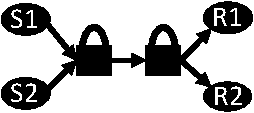
\includegraphics[width=0.15\textwidth]{images/one_conn3}
		\label{socksdirect:fig:fork-locking}
	}
	\hspace{0.02\textwidth}
	\subfloat[SocksDirect peer-to-peer]{
		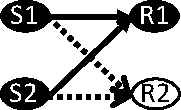
\includegraphics[width=0.11\textwidth]{images/one_conn1}
		\label{socksdirect:fig:fork-p2p}
	}
	\hspace{0.02\textwidth}
	\subfloat[S2 forks to S2' and S3]{
		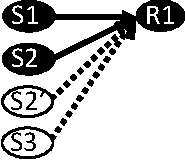
\includegraphics[width=0.1\textwidth]{images/one_conn2}
		\label{socksdirect:fig:fork-fork}
	}
	
	\caption{Inter-process queue architectures for a shared socket. Dashed arrows represent non-activated queues.}
\end{figure}
\fi

\begin{figure}[t!]
	\centering
	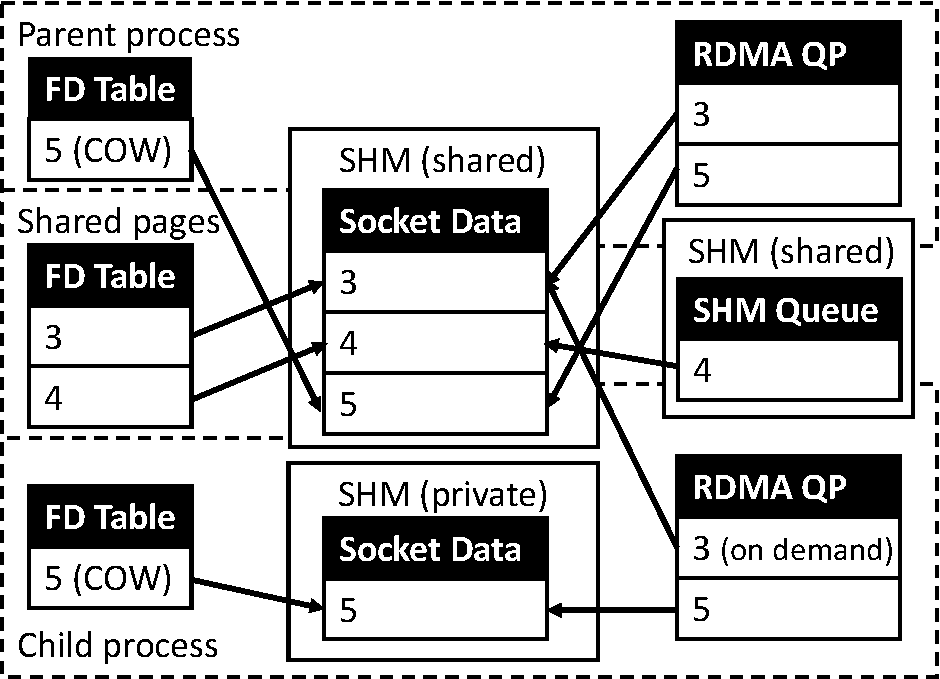
\includegraphics[width=0.6\textwidth]{images/fork_memory}
	
	\caption{Memory layout after fork. FDs 3 and 4 are created before fork and thus shared. After fork, parent and child processes each creates a new FD 5, which is copied on write in FD table. Socket metadata and buffers of FDs 3 and 4 are in SHM and thus shared. The child process creates a new SHM to store socket metadata and buffers of FD 5, which will be shared to its child when it forks again. RDMA QPs are in private memory, while SHM queues are shared.}
	\label{socksdirect:fig:fork-memory}
\end{figure}

\parab{Socket data sharing.}
The main challenge is to share socket metadata, buffers and underlying transports after \texttt{fork} and \texttt{exec}.
The memory space becomes copy-on-write after fork and is wiped after exec, but the socket FDs should still be usable.
We use shared memory (SHM) to store the socket metadata and buffers, so after fork, the data is still shared.
To attach the SHM after exec, \libipc{} connects to the monitor to fetch the SHM key of its parent process.
After fork, because a socket created by the child process is not visible by the parent, the child creates a new piece of SHM to store metadata and buffers of new sockets.

Now we need to share the underlying transports that are connected to peers.
SHM transport does not need special care, because a SHM created before fork/exec is still shared after fork/exec.
However, RDMA has problem with fork/exec because the DMA memory regions are not in SHM.
They become copy-on-write after fork, while the NIC still DMAs from the original physical pages, so the child process cannot use existing RDMA resources.
After exec, the entire RDMA context is wiped out.
Our solution is to let the child process re-initialize RDMA resources (PD, MR, etc.) after fork/exec.
When a child process uses a socket created before fork, it asks the monitor to re-establish an RDMA QP with the remote endpoint.
So, the remote may see two or more QPs for one socket, but they link to the unique copy of socket metadata and buffer.
Figure~\ref{socksdirect:fig:fork-memory} shows an example of fork.

\parab{FD space sharing.}
Different from socket data, the FD space becomes copy-on-write after fork: existing FDs are shared, but new FDs are exclusively owned by the creater process.
So the FD remapping table resides in heap memory, which is copy-on-write after fork.
To recover the FD remapping table after exec, it is copied to a shared memory before exec and attached to the new process during \libipc{} intialization.

\parab{Security.}
%Another challenge is to identify parent and child processes in the monitor.
Security is a concern because a malicious process may disguise itself as the child process of a privileged parent process.
To identify the parent and child relationship in the monitor, when an application calls \texttt{fork}, \texttt{clone} or \texttt{pthread\_create}, \libipc{} first generates a secret for pairing and sends it to the monitor, then invokes the original function in \emph{libc}.
After fork, the child process creates a new SHM queue to the monitor and sends the secret (child inherits parent memory space and knows the secret).
The monitor can thus pair the child process with the parent.

\parab{Monitor action.}
Upon fork, exec or thread creation, each existing socket needs to add a sender to the sending direction and a receiver to the receiving direction.
The parent process inherits the token, so the child process is always inactive.

%The socket queues are in SHM between parent and child processes.
%However, to avoid synchronization in accessing shared metadata, the metadata is in thread local storage and copied from parent to child.
%To maintain isolation between parent and child, monitor creates new shared memory queues to replace all queues in \emph{both} parent and child, as Figure~\ref{socksdirect:fig:fork-fork} shows. We do not reuse queues due to potential isolation violation. %The monitor then sends credentials of new queues to parent and child via bootstrap sockets. 
%Each peer process is notified of the new queues and the new process. From then on, parent and child processes have isolated queues to the monitor and peers.

%A harder challenge comes from socket connection sharing between parent and child processes.
%A major challenge is how to handle the remaining data in the original send and receive queues.

%For each unidirectional queue, we discuss the behavior of related processes in four cases:
%\begin{enumerate}
%	\item A sender process itself forks.
%	\item A receiver of a sender process forks.
%	\item A receiver process itself forks.
%	\item A sender of a receiver process forks.
%\end{enumerate}

%The general process of fork is that after monitor is notified of the fork, it creates shared memory between the newly created process and all the processes which previously have connections with the parent process. The key challenge lies in the fork is that how to deal with the existing data in the connection to guarantee the order requirements.

%\parab{Receiver fork.}
%First we look at a simple case when a receiver forks. Recall that only one receiver has exclusive access to a socket, as stated in Sec.~\ref{socksdirect:subsubsec:fork_rdwr}. The parent process inherits receive permission. When a sender receives fork notification of its peer, it copies all data from original queues to new queues of the parent process.

%\parab{Sender fork.}
%When a sender forks, things are more complicated. We need to guarantee that all data sent prior to \texttt{fork} is consumed before the data sent after \texttt{fork}.

%Our solution is to let receivers drain the original queue first before switching to the new queues. After \texttt{fork}, both parent and child send data to its new queue. When the receiver is notified of the fork, it keeps track of the original queue and consumes all data in it before activating new queues. Note that the parent or child may fork again before the original queue is drained. With this in mind, the receiver maintains a forest data structure to track dependency of queues. The root of each tree in the forest is the oldest queue to receive from. Each non-leaf node has two children indicating the new queue of parent and child processes. If a non-leaf root queue becomes empty, it will be removed, and the two children queues will be promoted to root nodes.

%\parab{Takeover During Fork.}
%After a sender forks, the receivers still need the takeover mechanism to arbitrate remaining messages in the original queue. However, both parent and child senders have dropped the original queue and will not respond to takeover requests. A similar situation occurs when a sender process dies. Our solution is to let the receivers use atomic operations to compete for remaining data in the original queue. Since this case rarely happens, the performance of the overall design is not affected.

%Things become much more complicated when cases 1,4 happens after cases 2,3 happening. After receiver forks, the unique sender is responsible for receiving ``takeover message'' and resend the data to new receivers. However, if sender forks following the receiver forks, according to the methods we mentioned above, there is no sender responsible for processing ``takeover message''. Our solution is that we require the receivers to poll the data from the old shared memory queue and compete for data. Since this case rarely happens, the performance of the overall design is not affected.

\subsubsection{Container Live Migration}
\label{socksdirect:subsubsec:container_live_migration}
\quad

\parab{Migration of remaining data in socket queues.}
Because \libipc{} runs in the same process with the application, its memory states are migrated to the new host together with the application.
The memory states include the socket queues, so the in-flight (sent but not received) data will not be lost.
A socket can be only shared within a container, and all processes in a container are migrated together, so memory on the original host can be de-allocated after migration.

\parab{Migration of monitor states.}
The monitor keeps track of listening socket information, active thread and waiting list of each connection, and shared memory secrets.
During migration, the old monitor dumps states of the migrated containers and sends them to the new monitor.

\parab{Establish new communication channels.}
After migration, all communication channels become obsolete because shared memory is local on a host and RDMA does not support live migration~\cite{nsdi19freeflow,slim}.
First, the migrated container on the new host needs to establish a connection to the local monitor.
The local monitor directs the following process.
An intra-host connection between two containers may become inter-host, so \libipc{} creates an RDMA connection in this case.
An inter-host connection between two containers may become intra-host, and \libipc{} creates a shared memory connection.
Finally, \libipc{} re-establishes remaining inter-host RDMA and intra-host shared memory connections.



%\subsubsection{Connection Creation}
%\label{socksdirect:subsubsec:fork_new}
%\quad

%A connection created by a thread can be accessed by all threads in the same process.
%To avoid creating redundant queues and connection states, \libipc does not share the FD eagerly with other threads, because most threads in existing applications do not use connections created by other threads.
%When a thread do want to accesses a FD that belongs to another thread, \libipc sends a message to the owner thread and requests sharing the FD. %This procedure is exactly the same as sharing existing connections during thread creation (Sec.~\ref{socksdirect:subsubsec:fork_fork}). %The sharing procedure only happens once for every connection and thread. Sharing existing connections eagerly during thread creation is an optimization. First, children threads are more likely to use existing connections than siblings. Second, batch processing improves performance.

%\subsubsection{Connection Close}
%\label{socksdirect:subsubsec:fork_close}
%\quad

%Close is the operation that all of the processes leave the connection. The synchronization is  especially challenging since all the processes are run in parallel. One challenge lies in file descriptors are managed by decentralized processes and are possibly reused. One process close a connection while the others are doing compute intensive tasks is a case. It is possible that the file descriptor of the old process is reused and a new connection is setup with the same file descriptor. The other process may notice the close of the old connection and also call close on its own side, which lead to the new connection setup by the previous process closed due to the match of same file descriptor. 

%To satisfy the synchronization requirements, the close function call is all completed by message passing. The caller of close need to wait for ACK from all the other peers before release resources. i.e. the status of the connection.

%\parab{Broadcast.}
%When a process calls \texttt{close}, all its peers cannot send to or receive from the FD. In this sense, 
%A socket is closed if all shared processes close it. So, we need to multicast a notification to the peers and collect responses from them. A challenge arises when \texttt{close} is interleaved with \texttt{fork}. Since \texttt{fork} and \texttt{close} do not commute~\cite{clements2015scalable}, we need a rule to determine their partial order. We make the choice that the ordering is determined by the initiator of \texttt{close}. If a process calls \texttt{close} before receiving fork notification, it will piggyback close notification with fork completion to both parent and child processes.

%\parab{Handshake before releasing resource.}
%Another challenge is caused by FD reuse after close. As stated in Sec.~\ref{socksdirect:subsec:socket-api}, a FD is deleted after receiving shutdown message of both directions. With multiple processes sharing a connection, after one process calls \texttt{close}, others can still use the connection. Consequently, a process deletes a FD only after receiving shutdown messages of both directions from all peers of the FD.

%Another challenge lies in the close of a connection is that close is a broadcast operation while send/receive is sent to a specific process. Besides, fork and close are immutable operations while the scalability requirements of the system impose the constraint that all the operations run asynchronously. As a result, a rule to determine the partial order is required.

%In \libipc, we make the choice that the order of fork and close is determined at the start point of the fork operation and the end point (after receiving all the ACKs). By making this choice, when a process waiting fork close ACK encounters fork message, it could send a separate close request to newly created process, which guarantees all the processes closed.

\iffalse
\subsection{Multiplex Sockets via One Queue}
\label{socksdirect:subsec:multiplex-conn}

\begin{figure}[t]
	\centering
	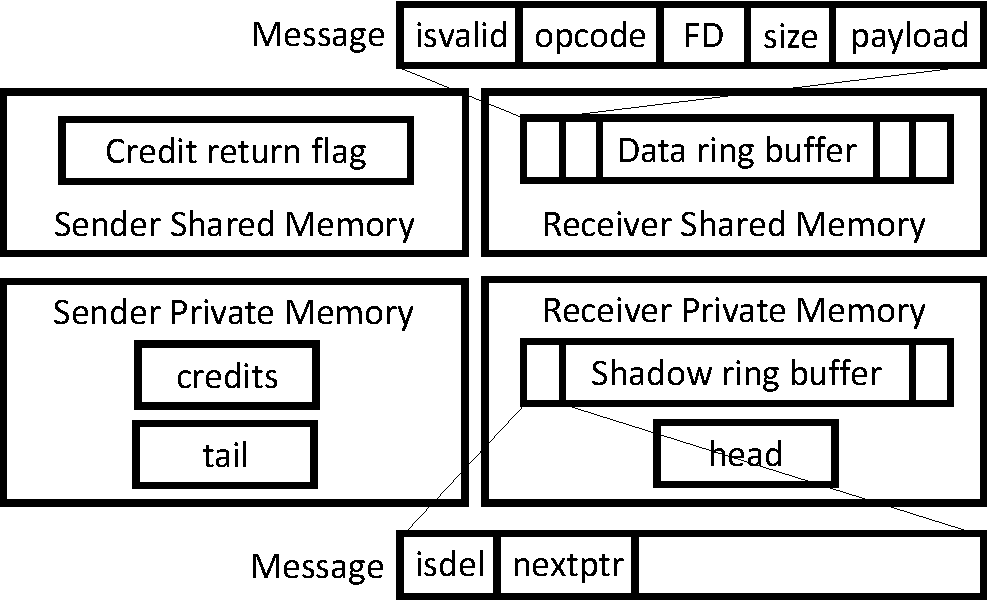
\includegraphics[width=0.4\textwidth]{images/locklessq_new}
	
	\caption{The structure of an inter-process queue.}
	
	\label{socksdirect:fig:locklessq-structure}
\end{figure}


%\parab{Multiplex connections in event-driven applications.}
To reduce memory footprint and improve locality of memory accesses, we use one queue to multiplex all connections between a pair of threads. Each data item in the queue is marked with its FD. By using a single queue, we reduce per-socket memory footprint, random memory accesses and cache misses.

\parab{Message format.}
As shown in Figure~\ref{socksdirect:fig:locklessq-structure}, the main component of the queue is a \emph{data ring buffer}, where messages are stored back-to-back.
Each message in the ring buffer consists of an 8-byte header and a variably sized payload. The header consists of an \textit{isvalid} flag, an opcode, the receiver's FD number and the payload size. Messages are aligned to 8 bytes to ensure header write atomicity.% and accelerate payload copy.

\parab{Event polling.}
We maintain a bitmap of each epoll FD set.
When \texttt{epoll\_wait} is called, we scan all data queues round-robin and check the FD of each data message against the bitmap. If the FD is in the bitmap, an event is returned to the application.
A global cursor exists to resume data queue scanning from the last position in the last scanned queue.

A per-queue cursor records the last scanned position in each queue to avoid scanning a message multiple times.
To speedup repeated receive operations of a specific FD, we build a linked list of messages for each FD as a side product of event polling.
Each FD maintains positions of the first and last scanned but unread messages of the FD.
When a new message of the FD is scanned, the \emph{nextptr} pointer in the last message is updated to point to the new message.

To poll events from sockets and other FDs (handled by kernel) at the same time, \libipc{} creates an \textit{epoll thread} in each process to wait on all FDs handled by kernel. When it receives a kernel event, it broadcasts the event to application threads via shared memory queues. %\texttt{Epoll\_wait} in \libipc{} will return such kernel events in addition to socket events. %Note that Linux allows an event to be received by multiple threads sharing the FD.

\parab{Pick from middle of queue.}
In order to support receiving data from a specific FD, the queue needs to support picking a message in the middle with a specific FD.
Fortunately, this does not happen frequently. Event-driven applications typically process incoming events in a FIFO order. For \texttt{epoll\_wait} in level trigger mode, we iterate through all messages in the queue and return those in the set of registered FDs. When applications call \texttt{recv}, \libipc{} would usually dequeue the message at head.

To pick from middle of queue, receiver traverses messages in the ring buffer. During traversal, receiver iterates messages from \textit{head} until free space in ring buffer, determined by \textit{isvalid}. Hence, receiver cannot clear \textit{isvalid} when a non-head message is dequeued. That's why each message has an \textit{isdel} flag. When a message is dequeued from the middle, its \textit{isdel} is set. %If the message at \textit{head} has \textit{isdel} set, the receiver advances \textit{head} and repeats this step.

\parab{Head-of-line blocking.}
%Second, if application does not receive from a FD for a long time, data items of the FD may fill up the queue and starve other FDs.
If application does not receive from a FD for a long time, the empty space in queue will become fragmented.
When data queue is full, the sender sends a message via emergency queue to trigger garbage collection in the receiver.
The receiver scans empty space in the middle of queue and moves remaining messages, so that empty space can be returned to the sender.
%To avoid starvation, we need at least one byte of headroom per FD. Accordingly, we design a single byte \textit{headroom slot} per FD. When data queue is full and the per-FD headroom slot is free, sender uses it and sends a notification via emergency queue. Receiver receives from data queue first, then from the headroom slot if it received a notification.

\parab{Emergency queue.}
Control messages may need to be delivered out-of-band when the queue is full. For example, in order to close the receive direction while sending data, the shutdown message should not be blocked by unconsumed data in the queue. To this end, we add an \textit{emergency queue} alongside each data queue.
A receiver will always retrieve messages in the emergency queue immediately.
\fi

